\documentclass[3p,authoryear]{elsarticle}

\usepackage{fontspec}
\usepackage[brazil]{babel}
\usepackage{microtype}
\usepackage{amsmath,amssymb}
\usepackage{icomma}
\usepackage{graphicx}
\usepackage{booktabs}
\usepackage{tabularx}
\usepackage{array}
\usepackage{multirow}
\usepackage{xcolor}
\usepackage{tikz}
\usetikzlibrary{arrows.meta,positioning}
\usepackage[american]{circuitikz}
\usepackage{enumitem}
\usepackage{caption}
\usepackage[hidelinks]{hyperref}

\captionsetup{font=small,labelfont=bf}
\setlist{itemsep=1pt,topsep=3pt}
\setlength{\emergencystretch}{2em}
\renewcommand{\topfraction}{0.9}
\renewcommand{\bottomfraction}{0.8}
\renewcommand{\textfraction}{0.07}
\renewcommand{\floatpagefraction}{0.75}
\setcounter{topnumber}{3}
\setcounter{bottomnumber}{2}
\setcounter{totalnumber}{4}

\definecolor{azul}{HTML}{1F5FA8}
\definecolor{verde}{HTML}{2E8B57}
\definecolor{vermelho}{HTML}{D1495B}
\definecolor{amarelo}{HTML}{EDAE49}
\definecolor{cinza}{HTML}{555555}

\newcommand{\vpv}{v_{\mathrm{pv}}}
\newcommand{\ipv}{i_{\mathrm{pv}}}
\newcommand{\Ipv}{I_{\mathrm{pv}}}
\newcommand{\Vt}{V_{\mathrm{t}}}
\newcommand{\Vref}{V_{\mathrm{ref}}}
\newcommand{\Vbat}{V_{\mathrm{bat}}}
\newcommand{\Tamb}{T_{\mathrm{amb}}}
\newcommand{\etaM}{\eta_{\mathrm{MPPT}}}

\abstracttitle{Resumo}
\keywordtitle{Palavras-chave}
\journal{DAS5109 -- Modelagem e Simulação de Processos (UFSC)}
\myfooter[L]{DAS5109 -- Modelagem e Simulação de Processos -- UFSC, 2026}

\begin{document}

\begin{frontmatter}

\title{Módulo fotovoltaico sob sombreamento parcial: modelagem eletrotérmica,
conversor buck-boost com perdas e comparação de algoritmos de MPPT local e global}

\author{Tiago Seemann}
\address{Universidade Federal de Santa Catarina, Departamento de Automação e Sistemas,
Florianópolis, Santa Catarina, Brasil}

\begin{abstract}
Este trabalho modela um módulo fotovoltaico comercial (ZTROON ZTP-160M, 160\,W) que carrega
uma bateria de 12\,V por meio de um conversor buck-boost, e compara três algoritmos de
rastreamento do ponto de máxima potência (MPPT): Perturba e Observa (P\&O), Condutância
Incremental (InC) e Enxame de Partículas (PSO). O módulo é descrito pelo modelo de dois
diodos, dividido em três submódulos com diodos de \emph{bypass}, o que reproduz as curvas
P-V com vários máximos típicas do sombreamento parcial. Ao modelo elétrico somam-se um
balanço térmico concentrado calibrado pelo NMOT ($k_h = 0{,}79$, $\tau \approx 7$\,min), um
modelo médio do conversor com perdas validado contra o modelo chaveado e uma malha PI de
tensão projetada por linearização, com margens verificadas em 56 casos de ponto de operação
e tolerância de componentes. Três achados de modelagem se destacam: o datasheet não
identifica a corrente de saturação do segundo diodo; o gap de energia precisa ser um
parâmetro efetivo ajustado pelo coeficiente $K_v$; e a formulação DAE com matriz de massa
falha em 9 de 36 simulações, o que levou a uma EDO reduzida de quatro estados. Sob sombra
estática, P\&O e InC ficam presos em picos locais (42 a 79\,\% do máximo global), enquanto o
PSO chega a mais de 99,99\,\%. No perfil dinâmico da norma EN~50530, sem sombra, o P\&O é o
melhor ($\etaM = 0{,}9992$) e o PSO o pior (0,9862). Num dia real de Florianópolis com
nuvens e sombra de poste sintéticas, o PSO entrega 941,7\,Wh à bateria, contra 913,4\,Wh do
P\&O e 896,5\,Wh do InC. A ablação mostra que ignorar o aquecimento do módulo superestima a
energia em cerca de 9\,\% e ignorar as perdas do conversor, em cerca de 11\,\%. As
simplificações do trabalho anterior, aplicadas ao mesmo dia, superestimam a energia na
bateria em 21,9\,\%.
\end{abstract}

\begin{keyword}
energia fotovoltaica \sep sombreamento parcial \sep modelo de dois diodos \sep buck-boost
\sep MPPT \sep enxame de partículas
\end{keyword}

\end{frontmatter}

% =====================================================================
\section{Introdução}
\label{sec:intro}

Um sistema fotovoltaico autônomo simples tem três partes em série: o módulo, um conversor
CC-CC e uma bateria. A potência que o módulo entrega depende do ponto da curva
corrente-tensão (I-V) em que ele opera, e para cada condição de irradiância e temperatura
existe um único ponto de máxima potência (MPP). Como esse ponto muda com o sol, com as
nuvens e com o aquecimento do módulo, o conversor é comandado por um algoritmo de
\emph{rastreamento do ponto de máxima potência} (MPPT), que ajusta continuamente a tensão de
operação \citep{esram}.

O problema se complica quando o módulo é sombreado só em parte. As células estão em série e
são protegidas por diodos de \emph{bypass}; quando um grupo de células recebe menos luz, o
seu diodo conduz e a curva potência-tensão (P-V) passa a ter vários máximos locais
\citep{patel}. Algoritmos de subida de encosta, como o P\&O e a Condutância Incremental,
param no primeiro máximo que encontram, que pode não ser o global. Algoritmos de busca
global, como o PSO \citep{kennedy,ishaquepso}, exploram a faixa de tensão inteira, mas
gastam energia durante a exploração.

\paragraph{O trabalho anterior.} No semestre anterior, \citet{anterior} modelaram o mesmo
módulo (ZTROON ZTP-160M) com um conversor buck-boost em MATLAB. Eles usaram o modelo de um
diodo, com três parâmetros ($R_s$, $R_p$ e a corrente de saturação) ajustados pelo
\texttt{fsolve} a partir do ponto de máxima potência, e obtiveram valores sem significado
físico ($R_s \approx 9\times10^{-16}\,\Omega$, corrente de saturação $\approx
4\times10^{-20}$\,A). A temperatura entrava como valor fixo (0, 25 ou 60\,°C, com
temperatura de referência de 278\,K em vez de 298\,K) e o conversor era ideal, com
$f_s = 2$\,kHz, $L = 1$\,mH e $C = 800\,\mu$F. Um PI de tensão e um P\&O foram ajustados por
tentativa e testados com dois degraus de irradiância uniforme (1000 $\to$ 500 $\to$
800\,W/m²) em cerca de 1\,s de simulação. A conclusão foi qualitativa: o P\&O ``garante que a
potência máxima seja entregue à carga''. Não houve sombreamento parcial, modelo térmico,
perdas, nem métrica de eficiência.

\paragraph{Pergunta central.} \emph{Quanta energia o P\&O deixa de captar quando há
sombreamento parcial, e quanto um método de busca global (PSO) consegue recuperar,
considerando o aquecimento do módulo e as perdas do conversor?}

\paragraph{Contribuições.} A Tabela~\ref{tab:comparacao} resume o que muda em relação ao
trabalho anterior. Em particular, este trabalho:
\begin{enumerate}[label=(\roman*)]
\item extrai os parâmetros do modelo de dois diodos com cinco condições do datasheet, mostra
que o segundo diodo não é identificável e valida o modelo com um dado que não entra no
ajuste (o coeficiente térmico de $P_{max}$);
\item acopla um modelo térmico calibrado pelo NMOT e um conversor com perdas, validado
contra o modelo chaveado;
\item projeta o PI por linearização e margens, com robustez a tolerâncias de componentes,
e deriva o período do MPPT da dinâmica da malha \citep{femia};
\item organiza a simulação numa hierarquia de modelos (chaveado, médio e quase-estático),
validando cada simplificação contra o nível mais detalhado;
\item compara P\&O, InC e PSO por métricas de energia sob sombra estática, no perfil
dinâmico da norma EN~50530 e num dia real, e mede quanto cada simplificação do trabalho
anterior distorce a energia calculada.
\end{enumerate}

\begin{table}[!htbp]
\centering\small
\renewcommand{\arraystretch}{1.15}
\begin{tabularx}{\linewidth}{>{\bfseries}l X X}
\toprule
Bloco & Trabalho anterior \citep{anterior} & Este trabalho \\
\midrule
Painel & 1 diodo; 3 parâmetros ajustados pelo MPP ($R_s\approx10^{-16}\,\Omega$) &
2 diodos; 5 condições do datasheet; análise de identificabilidade; $R_p(G)$ \\
Sombra & Irradiância uniforme & 3 submódulos com \emph{bypass}; curvas com vários picos \\
Temperatura & Fixa (0, 25, 60\,°C) & EDO de balanço de energia calibrada pelo NMOT \\
Conversor & Ideal, médio, 2\,kHz & Médio com perdas, 20\,kHz, validado contra o chaveado;
verificação de CCM/DCM \\
Controle & PI e P\&O por tentativa & PI por margens em 56 casos; período do MPPT por
\citet{femia} \\
MPPT & P\&O & P\&O, InC e PSO, com o mesmo período e a mesma malha interna \\
Testes & 2 degraus de $G$ em $\approx$1\,s & Sombra estática; EN~50530 ($\approx$7\,h); dia
real com sombras \\
Resultado & Qualitativo & Eficiência de rastreamento, energia na bateria, ablação \\
\bottomrule
\end{tabularx}
\caption{Do trabalho anterior para este. O módulo (ZTP-160M) e a ferramenta (MATLAB, aqui
sem \emph{toolboxes}) são os mesmos, o que permite usar o trabalho anterior como linha de
base (Seção~\ref{sec:e8}).}
\label{tab:comparacao}
\end{table}

O texto segue a ordem do modelo. A Seção~\ref{sec:fund} apresenta a física de cada bloco; a
Seção~\ref{sec:metodos}, os métodos numéricos e as decisões de modelagem; a
Seção~\ref{sec:validacao}, a validação de cada bloco; a Seção~\ref{sec:resultados}, os
resultados; e a Seção~\ref{sec:conclusao} responde à pergunta central e lista as limitações.

% =====================================================================
\section{Fundamentação}
\label{sec:fund}

A Figura~\ref{fig:blocos} mostra o sistema. O conversor impõe a tensão do módulo e o
módulo devolve a corrente; a temperatura altera a parte elétrica e a potência elétrica
extraída altera o balanço térmico. O MPPT escolhe a referência de tensão $\Vref$ e o PI
manipula a razão cíclica $d$ para levar o módulo até ela.

\begin{figure}[!htbp]
\centering
\begin{tikzpicture}[
  bloco/.style={draw,rounded corners,minimum width=2.6cm,minimum height=1.0cm,align=center,thick,font=\small},
  seta/.style={-{Stealth[length=2.4mm]},thick},
  lbl/.style={font=\footnotesize,midway}]
\node[bloco,fill=cinza!10] (clima) at (0,2.2) {Clima\\$G_j(t)$, $\Tamb(t)$, vento};
\node[bloco,fill=amarelo!25] (pv) at (0,0) {Módulo\\2 diodos + \emph{bypass}};
\node[bloco,fill=vermelho!12] (term) at (-4,0) {Térmico\\$T(t)$};
\node[bloco,fill=azul!12] (conv) at (4.2,0) {Buck-boost\\com perdas};
\node[bloco,fill=verde!15] (bat) at (8,0) {Bateria\\$\Vbat=12$\,V};
\node[bloco,fill=azul!5] (pi) at (4.2,-2.3) {PI de tensão};
\node[bloco,fill=azul!5] (mppt) at (0,-2.3) {MPPT\\P\&O / InC / PSO};
\draw[seta] (clima) -- (pv);
\draw[seta] (clima.west) -| (term.north);
\draw[seta] ([yshift=2mm]term.east) -- node[lbl,above]{$T$} ([yshift=2mm]pv.west);
\draw[seta] ([yshift=-2mm]pv.west) -- node[lbl,below]{$P_{el}$} ([yshift=-2mm]term.east);
\draw[seta] ([yshift=2mm]pv.east) -- node[lbl,above]{$\ipv$} ([yshift=2mm]conv.west);
\draw[seta] ([yshift=-2mm]conv.west) -- node[lbl,below]{$\vpv$} ([yshift=-2mm]pv.east);
\draw[seta] (conv) -- (bat);
\draw[seta] (pv.south) -- node[lbl,left]{$\vpv,\ \ipv$} (mppt.north);
\draw[seta] (mppt) -- node[lbl,above]{$\Vref$} (pi);
\draw[seta] (pi) -- node[lbl,right]{$d$} (conv);
\end{tikzpicture}
\caption{Diagrama de blocos do sistema. $G_j$ é a irradiância de cada submódulo; os pares
de setas mostram os dois acoplamentos bidirecionais (módulo--conversor e
módulo--térmico).}
\label{fig:blocos}
\end{figure}

\subsection{Modelo de dois diodos}
\label{sec:2d}

Uma célula de silício é uma junção P-N. A luz gera uma fotocorrente $\Ipv$, proporcional à
irradiância $G$, mas a junção também é um diodo, e parte da corrente volta por ela. No
modelo de dois diodos (Figura~\ref{fig:circuitos}), um diodo representa a corrente de
difusão (fator de idealidade $a_1 \approx 1$) e outro a de recombinação na região de
depleção ($a_2 > 1$), que pesa mais em baixa tensão e pouca luz \citep{ishaque}. A Lei de
Kirchhoff das correntes dá, para $N_s$ células em série,
\begin{equation}
I = \Ipv
 - I_{01}\!\left[\exp\!\left(\frac{V+R_sI}{a_1 N_s\Vt}\right)-1\right]
 - I_{02}\!\left[\exp\!\left(\frac{V+R_sI}{a_2 N_s\Vt}\right)-1\right]
 - \frac{V+R_sI}{R_p},
\qquad \Vt = \frac{kT}{q},
\label{eq:2d}
\end{equation}
em que $R_s$ representa as perdas ôhmicas e $R_p$ as fugas. O clima entra por
\begin{align}
\Ipv(G,T) &= \frac{G}{G_n}\Big[I_{pv,n} + K_i\,(T-T_n)\Big], \label{eq:ipv}\\
I_{0k}(T) &= I_{0k,n}\left(\frac{T}{T_n}\right)^{3}
  \exp\!\left[\frac{q\,E_{g,\mathrm{ef}}}{k}\left(\frac{1}{T_n}-\frac{1}{T}\right)\right],
  \quad k=1,2, \label{eq:i0}\\
R_p(G) &= R_{p,\mathrm{ref}}\,\frac{G_n}{G}, \label{eq:rp}
\end{align}
com $G_n = 1000$\,W/m² e $T_n = 298{,}15$\,K. Duas escolhas merecem nota. Em
\eqref{eq:i0}, $E_{g,\mathrm{ef}}$ é um gap \emph{efetivo}, ajustado pelo coeficiente
térmico de $V_{oc}$ (Seção~\ref{sec:extracao}). Em \eqref{eq:rp}, a resistência paralela cai
com a luz, como propõem \citet{desoto}; com $R_p$ constante a fuga $V/R_p$ quase não muda
quando a fotocorrente cai, e em baixa irradiância vira uma fração exagerada da corrente.

\begin{figure}[!htbp]
\centering
\begin{circuitikz}[scale=0.78, transform shape]
\draw (0,0) to[I, l=$I_{pv}$] (0,3) -- (4.6,3);
\draw (1.4,3) to[D, l_=$D_1$] (1.4,0);
\draw (2.9,3) to[D, l_=$D_2$] (2.9,0);
\draw (4.4,3) to[R, l_=$R_p$] (4.4,0);
\draw (4.4,3) to[R, l=$R_s$, i=$I$, -o] (7.2,3);
\draw (0,0) to[short, -o] (7.2,0);
\draw (7.2,3) to[open, v^>=$V$] (7.2,0);
\node at (3.6,-0.8) {\small (a) modelo de 2 diodos};
\end{circuitikz}
\hspace{0.9cm}
\begin{circuitikz}[scale=0.78, transform shape]
\draw (0,0) to[I, l=$\text{sub.\,1}\ (G_1)$] (0,2.4);
\draw (2.2,0) to[D, l_=$D_{bp,1}$] (2.2,2.4);
\draw (0,2.4) to[I, l=$\text{sub.\,2}\ (G_2)$] (0,4.8);
\draw (2.2,2.4) to[D, l_=$D_{bp,2}$] (2.2,4.8);
\draw (0,0) -- (2.2,0);
\draw (0,2.4) -- (2.2,2.4);
\draw (0,4.8) -- (2.2,4.8);
\draw (2.2,4.8) to[short, -o] (3.8,4.8);
\draw (2.2,0) to[short, -o] (3.8,0);
\draw (3.8,4.8) to[open, v^>=$\vpv$] (3.8,0);
\node at (1.6,-0.8) {\small (b) submódulos com \emph{bypass}};
\end{circuitikz}
\caption{(a) Circuito equivalente de um grupo de células no modelo de dois diodos.
(b) Submódulos em série, cada um com seu diodo de \emph{bypass} (dois desenhados; o
ZTP-160M tem três): todos são atravessados pela mesma corrente e $\vpv = \sum_j V_j$.}
\label{fig:circuitos}
\end{figure}

\subsection{\texorpdfstring{Submódulos, \emph{bypass} e múltiplos picos}{Submódulos, bypass e múltiplos picos}}

As células em série são atravessadas pela mesma corrente. Se uma delas recebe menos luz e
a corrente imposta passa da que ela gera, ela é forçada à polarização reversa e dissipa
potência. O diodo de \emph{bypass}, em antiparalelo com cada grupo de células
(\emph{submódulo}), conduz quando a tensão do grupo tenta ficar negativa e a limita a
cerca de $-0{,}4$\,V. Com $N_{sub}$ submódulos, cada um com sua irradiância $G_j$ e sua
tensão $V_j$, as equações do módulo são
\begin{align}
I &= I_{c,j}(V_j, G_j, T) + I_{bp}(V_j), \qquad j = 1,\dots,N_{sub}, \label{eq:kcl}\\
I_{bp}(V_j) &= I_{0,bp}\left[\exp\!\left(\frac{-V_j}{n_{bp}\Vt}\right)-1\right], \label{eq:bp}\\
\vpv &= \sum_{j=1}^{N_{sub}} V_j, \label{eq:kvl}
\end{align}
em que $I_{c,j}$ é a equação~\eqref{eq:2d} aplicada às $N_s/N_{sub}$ células do
submódulo $j$. O \emph{bypass} é um diodo exponencial (e não um corte do tipo
$\max(V_j, -V_F)$) porque uma função suave preserva a convergência do método de Newton.

Com um submódulo sombreado, em corrente baixa os três geram e a tensão é alta; em corrente
alta o sombreado é desviado pelo \emph{bypass} e só os outros dois geram. Cada regime tem seu
máximo de potência, e a curva P-V passa a ter até $N_{sub}$ picos. Qual deles é o global
depende da intensidade da sombra (Seção~\ref{sec:e2}).

\subsection{Balanço térmico}

O módulo converte em eletricidade só cerca de 20\,\% da luz que recebe; o resto aquece as
células, e a potência cai cerca de 0,4\,\%/K. Como o módulo é fino e conduz calor
internamente muito mais rápido do que troca calor com o ar, ele é tratado como um único corpo
de temperatura uniforme $T$ (capacitância térmica concentrada). O balanço de energia é
\begin{equation}
m c_p \frac{dT}{dt} = \alpha A G - P_{el}
 - k_h\,h_w\,(2A)\,(T-\Tamb)
 - \varepsilon\sigma A\,(T^4 - T_{\text{céu}}^4)
 - \varepsilon\sigma A\,(T^4 - \Tamb^4),
\label{eq:termico}
\end{equation}
\begin{equation}
h_w = 2{,}8 + 3{,}0\,v_w \ \ [\mathrm{W/(m^2K)}], \qquad
T_{\text{céu}} = 0{,}0552\,\Tamb^{1{,}5} \ \ [\mathrm K],
\label{eq:correlacoes}
\end{equation}
com absortância $\alpha = 0{,}9$, emissividade $\varepsilon = 0{,}85$, área $A = 0{,}82$\,m²
e vento $v_w$. A convecção usa a correlação de \citet{watmuff} nas duas faces, e a radiação
de onda longa vai da face frontal para o céu \citep{swinbank} e da traseira para o solo, a
uma temperatura próxima de $\Tamb$ \citep{duffie}. O termo $P_{el}$ acopla as duas partes: a
energia que vira eletricidade não aquece o módulo. A capacidade térmica vem da massa do
datasheet, $m c_p / A = 8{,}9\,\text{kg}\times 840\,\text{J/(kg\,K)} / 0{,}82\,\text{m}^2
\approx 9{,}1$\,kJ/(m²K), e $k_h$ é um fator de correção da convecção, calibrado pelo NMOT
(Seção~\ref{sec:val_termico}).

\subsection{Conversor buck-boost}

O conversor (Figura~\ref{fig:buckboost}) alterna duas configurações a cada período
$T_s = 1/f_s$. Com a chave fechada (fração $d$), o indutor se carrega com a tensão do
módulo; com ela aberta, descarrega na bateria pelo diodo. Com $q(t)\in\{0,1\}$ indicando o
estado da chave, o \textbf{modelo chaveado} é
\begin{align}
q=1:\quad & L\frac{di_L}{dt} = \vpv - i_L(r_L+R_{on}), &
            & C\frac{d\vpv}{dt} = \ipv - i_L, \label{eq:chav1}\\
q=0:\quad & L\frac{di_L}{dt} = -(\Vbat+V_F) - i_L(r_L+R_D), &
            & C\frac{d\vpv}{dt} = \ipv, \label{eq:chav0}
\end{align}
com $i_L \ge 0$ (o diodo bloqueia corrente reversa). Trocando $q$ pela sua média $d$ num
período, obtém-se o \textbf{modelo médio com perdas} \citep{erickson,barbi}:
\begin{align}
L\frac{di_L}{dt} &= d\,\vpv - (1-d)(\Vbat+V_F) - i_L\big[r_L + d\,R_{on} + (1-d)R_D\big],
\label{eq:medio1}\\
C\frac{d\vpv}{dt} &= \ipv(\vpv) - d\,i_L. \label{eq:medio2}
\end{align}
No equilíbrio, $i_L = \ipv/d$, e substituindo em \eqref{eq:medio1} resulta uma equação do
segundo grau em $d$ com exatamente uma raiz positiva; sem perdas, $\Vbat/\vpv =
d/(1-d)$. A perda de chaveamento, $P_{sw} = \tfrac12(\vpv+\Vbat)\,i_L\,(t_r+t_f)\,f_s$, entra
só no balanço de potência. A topologia é necessária aqui: sem sombra o MPP fica em
19,6\,V (acima dos 12\,V da bateria, modo abaixador), mas com sombra o pico global pode cair
para 6 a 13\,V (Tabela~\ref{tab:picos}), e o conversor precisa elevar a tensão.

O modelo médio vale em condução contínua (CCM), isto é, enquanto
$i_L > \Delta i_L/2$, com $\Delta i_L = \vpv d/(L f_s)$. Em baixa irradiância a corrente cai,
o indutor zera a cada período (DCM) e as equações~\eqref{eq:medio1}--\eqref{eq:medio2}
deixam de valer.

\begin{figure}[!htbp]
\centering
\begin{circuitikz}[scale=0.85, transform shape]
\draw (0,0) to[I, l=$i_{pv}$] (0,3) -- (1.8,3);
\draw (1.8,3) to[C, l_=$C$, v^>=$v_{pv}$] (1.8,0);
\draw (1.8,3) to[spst, l=$S$] (4.2,3);
\draw (4.2,3) to[L, l_=$L$, i>^=$i_L$] (4.2,0);
\draw (6.8,3) to[D, l_=$D$] (4.2,3);
\draw (6.8,3) to[battery1, l_=$V_{bat}$] (6.8,0);
\draw (0,0) -- (6.8,0);
\node[font=\small] at (7.35,2.75) {$-$};
\node[font=\small] at (7.35,0.25) {$+$};
\end{circuitikz}
\caption{Buck-boost inversor. O módulo e o capacitor $C$ estão na entrada; a chave $S$ é
comandada por PWM com razão cíclica $d$. Perdas: $r_L$ (indutor), $R_{on}$ (MOSFET),
$V_F$ e $R_D$ (diodo Schottky) e chaveamento.}
\label{fig:buckboost}
\end{figure}

\subsection{Algoritmos de MPPT e métrica}
\label{sec:fund_mppt}

Os três algoritmos atuam sobre a mesma referência $\Vref$, com o mesmo período de amostragem
$T_a$ e a mesma malha PI.

\textbf{P\&O.} É uma subida de encosta: a referência anda um passo $\delta$; se a potência
subiu, continua no mesmo sentido, senão inverte,
\begin{equation}
\Vref[k+1] = \Vref[k] + \delta\,\operatorname{sinal}\big(\Delta P[k]\,\Delta V[k]\big).
\label{eq:po}
\end{equation}
Em regime oscila em três níveis em torno do MPP, e a perda por oscilação cresce com
$\delta^2$ \citep{femia}.

\textbf{InC.} Parte da condição exata de máximo, $dP/dV = I + V\,dI/dV = 0$
\citep{hussein}. Com $s = \Delta I/\Delta V + I/V$, a referência sobe se $s > \varepsilon$,
desce se $s < -\varepsilon$ e fica parada se $|s| \le \varepsilon$. Ao contrário do P\&O, pode
parar no MPP; como ele, só enxerga a inclinação local.

\textbf{PSO.} Cada partícula $i$ é uma tensão candidata $x_i$, que se move segundo
\citep{kennedy}
\begin{align}
v_i &\leftarrow w\,v_i + c_1 r_1\,(p_{best,i}-x_i) + c_2 r_2\,(g_{best}-x_i), \label{eq:pso1}\\
x_i &\leftarrow x_i + v_i, \label{eq:pso2}
\end{align}
com $r_1, r_2 \sim \mathcal U(0,1)$. O termo de inércia mantém o movimento, o segundo puxa
cada partícula para o melhor ponto que ela já viu e o terceiro para o melhor do enxame. Como
há um só módulo, as partículas são avaliadas uma por período $T_a$. Quando todas ficam perto
de $g_{best}$, a referência é fixada nele; se a potência medida mudar mais de 10\,\%, a busca
recomeça \citep{ishaquepso2}.

\textbf{Métrica.} A eficiência de rastreamento compara a energia extraída com a do máximo
\emph{global} disponível,
\begin{equation}
\etaM = \frac{\int P_{pv}(t)\,dt}{\int P_{mp,\mathrm{global}}(t)\,dt},
\label{eq:eta}
\end{equation}
em que $P_{mp,\mathrm{global}}(t)$ (o \emph{oráculo}) é calculado por varredura do modelo
estático. Com o máximo local no denominador, um P\&O preso no pico errado pareceria quase
perfeito. A energia na bateria, que desconta as perdas do conversor, é a métrica que
interessa ao usuário.

% =====================================================================
\section{Modelagem e métodos numéricos}
\label{sec:metodos}

Todo o código usa só o núcleo do MATLAB, sem as \emph{toolboxes} de Otimização e de
Controle. Por isso o ajuste por mínimos quadrados, a resposta em frequência e o cálculo de
margens foram implementados à mão, cada um com testes automatizados.

\subsection{Extração de parâmetros: um problema bem posto e um mal posto}
\label{sec:extracao}

O fabricante não informa $R_s$, $R_p$ e as correntes de saturação. O trabalho anterior impôs
essencialmente uma condição a três incógnitas; o sistema era subdeterminado e o
\texttt{fsolve} parou numa solução degenerada. Aqui, com $a_1 = 1$, $a_2 = 1{,}2$ e
$I_{01} = I_{02}$ \citep{ishaque}, as incógnitas são
$\boldsymbol\theta = [I_{pv,n},\ \log_{10} I_{01,n},\ R_s,\ R_p,\ E_{g,\mathrm{ef}}]$ e as
condições, tiradas do datasheet \citep{ztp160m}, são cinco:
\begin{equation}
I(0) = I_{sc},\quad I(V_{oc}) = 0,\quad I(V_{mp}) = I_{mp},\quad
\left.\frac{dP}{dV}\right|_{mp} = 0,\quad \frac{\partial V_{oc}}{\partial T} = K_v.
\label{eq:condicoes}
\end{equation}
A derivada $dI/dV$ sai por diferenciação implícita de \eqref{eq:2d}. O sistema $5\times5$ é
resolvido por Levenberg--Marquardt \citep{marquardt} com limites (cada passo é projetado de
volta na caixa de valores físicos) e com as variáveis normalizadas pela diagonal da matriz
normal, já que as incógnitas vão de $10^{-11}$\,A a $10^{1}\,\Omega$. A corrente de saturação
é ajustada em $\log_{10}$. Os limites tornam impossível a solução degenerada do trabalho
anterior.

\paragraph{Benchmark.} O mesmo código, aplicado ao módulo KC200GT, reproduz o modelo de um
diodo de \citet{villalva}: $R_s = 0{,}231\,\Omega$ contra $0{,}221\,\Omega$ publicado, e
$I_{pv}$ e $I_0$ dentro de 1\,\% e 5\,\%.

\paragraph{Dois achados.} Primeiro, \textbf{o datasheet não identifica o segundo diodo}:
fixando $I_{02}/I_{01}$ entre $10^{-2}$ e $10^{2}$, as cinco condições fecham com resíduo
abaixo de $10^{-7}$ (Tabela~\ref{tab:ident}), mas as previsões fora do ponto de referência
mudam. Por isso a razão é fixada por uma hipótese publicada \citep{ishaque}, e a faixa de
previsões vira a incerteza do modelo (Seção~\ref{sec:val_painel}). Segundo, \textbf{o gap
precisa ser efetivo}: com $E_g = 1{,}12$\,eV (silício), o modelo do KC200GT dá
$K_v = -0{,}106$\,V/K, contra $-0{,}123$\,V/K medido. Tratar $E_g$ como incógnita e impor
$K_v$ fecha o sistema; o valor obtido, 1,30\,eV no ZTP-160M, é um parâmetro de calibração da
lei~\eqref{eq:i0}, não o gap físico. A Tabela~\ref{tab:params} lista os parâmetros finais.

\begin{table}[!htbp]
\centering\small
\begin{tabular}{lcc}
\toprule
Parâmetro (módulo, 33 células) & 2 diodos & 1 diodo \\
\midrule
$I_{pv,n}$ [A] & 9,029 & 9,024 \\
$I_{01,n}$ [A] & $2{,}12\times10^{-11}$ & $2{,}44\times10^{-10}$ \\
$I_{02,n}$ [A] & $2{,}12\times10^{-11}$ & -- \\
$a_1$; $a_2$ & 1; 1,2 & 1,1; -- \\
$R_s$ [$\Omega$] & 0,042 & 0,019 \\
$R_{p,\mathrm{ref}}$ [$\Omega$] & 40,9 & 43,7 \\
$E_{g,\mathrm{ef}}$ [eV] & 1,304 & 1,182 \\
\bottomrule
\end{tabular}
\caption{Parâmetros extraídos do datasheet do ZTP-160M ($P_{max} = 160$\,W,
$V_{mp} = 19{,}57$\,V, $I_{mp} = 8{,}20$\,A, $V_{oc} = 22{,}64$\,V, $I_{sc} = 9{,}02$\,A,
$K_v = -0{,}34$\,\%/K, $K_i = +0{,}05$\,\%/K). No modelo de um diodo, $a = 1{,}1$ é o maior
valor (em passos de 0,1) que ajusta este módulo sem $R_s \le 0$.}
\label{tab:params}
\end{table}

\subsection{Corrente do módulo sombreado: Newton com jacobiano analítico}

Dada a tensão $\vpv$ imposta pelo conversor, as equações~\eqref{eq:kcl}--\eqref{eq:kvl} formam
um sistema de $N_{sub}+1$ equações. A escolha das incógnitas importa. Usando a tensão de
junção de cada submódulo, $V_{d,j} = V_j + R_s I_{c,j}$, em vez de $V_j$, a corrente das
células fica explícita,
$I_{c,j} = \Ipv - I_{01}(e^{V_{d,j}/a_1\Vt'} - 1) - I_{02}(e^{V_{d,j}/a_2\Vt'} - 1) -
V_{d,j}/R_p$ (com $\Vt'$ a tensão térmica do grupo), e as incógnitas
$\mathbf z = [I, V_{d,1}, \dots, V_{d,N_{sub}}]$ satisfazem
\begin{equation}
R_j(\mathbf z) = I_{c,j} + I_{bp,j} - I = 0,\qquad
R_{N_{sub}+1}(\mathbf z) = \sum_j \big(V_{d,j} - R_s I_{c,j}\big) - \vpv = 0.
\label{eq:residuo}
\end{equation}
O jacobiano é analítico e tem forma de seta: cada equação de submódulo depende só de $I$ e
do seu $V_{d,j}$. O passo de Newton é limitado a $2\Vt'$ em $V_{d,j}$ para evitar
\emph{overflow} das exponenciais longe da solução, e a solução do instante anterior serve
de chute inicial (\emph{warm start}). A tolerância é $10^{-9}$ no resíduo.

\subsection{Formulação dinâmica: da DAE à EDO reduzida}
\label{sec:edo}

O modelo médio acoplado ao módulo é naturalmente uma DAE: estados diferenciais
$[\vpv, i_L]$ e restrições algébricas \eqref{eq:residuo}. A primeira formulação entregou
tudo ao \texttt{ode15s} \citep{shampine} com uma matriz de massa singular,
$M = \operatorname{diag}(1,1,0,\dots,0)$. Em malha aberta funcionou, desde que com o
jacobiano analítico (com diferenças finitas, a exponencial do \emph{bypass} fazia o
integrador falhar). Em malha fechada com MPPT, porém, a DAE \textbf{falhou em 9 dos 36
casos} de teste, sempre nos degraus grandes de referência do PSO sob sombra. O
\texttt{ode15s} reaproveita o jacobiano por vários passos, e a condutância dos diodos varia
exponencialmente (de $10^{-2}$ a $10^{2}$\,S) quando o ponto de operação cruza o joelho de um
submódulo; um jacobiano velho leva o Newton interno do integrador a divergir.

A formulação final é uma \textbf{EDO reduzida} de quatro estados,
\begin{equation}
\mathbf x = [\vpv,\ i_L,\ \xi,\ T], \qquad
\dot{\mathbf x} = \mathbf f\big(\mathbf x, I(\mathbf x)\big),
\label{eq:edo}
\end{equation}
em que $\xi$ é a integral do erro do PI e a corrente $I(\vpv, G, T)$ é resolvida pelo Newton
da seção anterior a cada avaliação de $\mathbf f$. O jacobiano de $\mathbf f$ usa a regra da
cadeia, com $dI/d\vpv$ e $dI/dT$ obtidos por diferenciação implícita de \eqref{eq:residuo}.
O resultado: 0 falhas em 36 casos, eficiências iguais às da DAE em quatro dígitos nos casos
em que ambas convergem, ao custo de 2 a 4 vezes mais CPU (1 a 2,5\,s por segundo simulado).
O \texttt{ode15s} continua necessário, porque o sistema é rígido: a ressonância LC
($\sim$240\,Hz) convive com o térmico (minutos).

\subsection{Hierarquia de modelos e escalas de tempo}
\label{sec:hierarquia}

Os fenômenos vão do chaveamento (50\,$\mu$s) ao dia solar (13\,h). Simular um dia inteiro
com o modelo chaveado é inviável; por isso cada experimento usa o nível de detalhe
suficiente (Tabela~\ref{tab:hierarquia}), e cada simplificação é validada contra o nível
acima num intervalo em que ambos rodam (Seções~\ref{sec:e3} e~\ref{sec:val_qe}).

\begin{table}[!htbp]
\centering\small
\begin{tabularx}{\linewidth}{l X l l}
\toprule
Modelo & Formulação e passo & Uso & Custo de CPU \\
\midrule
Chaveado & Euler explícito, passo $T_s/200$; Newton do painel a cada passo &
Validar o médio (E3) & $\sim$1--2\,s por 6\,ms \\
Médio dinâmico & EDO reduzida \eqref{eq:edo}, \texttt{ode15s}, MPPT a cada $T_a$ &
Transitórios (E4, trecho do E6) & 1--2,5\,s por s \\
Quase-estático & Conversor e PI em regime a cada $T_a$; térmico por Euler com passo $T_a$;
oráculo a cada 1\,s & EN~50530, dia (E6--E8) & $\sim$65\,s por hora \\
\bottomrule
\end{tabularx}
\caption{Hierarquia de modelos. Os custos são os medidos no desenvolvimento (decisões D15 e
D16 do plano do trabalho).}
\label{tab:hierarquia}
\end{table}

No \textbf{modelo quase-estático}, como o PI acomoda em menos de um período do MPPT
($T_a = 1{,}5\,t_s$, Seção~\ref{sec:pi}), cada período é tratado como regime permanente: a
tensão do módulo é $\Vref$, a potência é $\Vref\, I(\Vref)$ e as perdas saem da solução
fechada do equilíbrio do conversor. O térmico, com constantes de tempo de minutos, é
integrado por Euler com passo $T_a \approx 31$\,ms, milhares de vezes menor. O oráculo é a
parte cara: avaliado a cada 1\,s (regra do ponto médio por bloco), custa $\sim$65\,s de CPU
por hora simulada, contra $\sim$2500\,s se avaliado a cada $T_a$.

\subsection{Linearização e projeto do PI}
\label{sec:pi}

Em torno de um equilíbrio, o módulo se comporta como uma resistência dinâmica
$r_{pv} = -dV/dI$; no MPP vale $r_{pv} = V_{mp}/I_{mp}$. Linearizando
\eqref{eq:medio1}--\eqref{eq:medio2} sem perdas, obtém-se
\begin{equation}
G_{vd}(s) = \frac{\tilde v_{pv}(s)}{\tilde d(s)}
= -\,\frac{L\,I_L\,s + D\,(V_{pv}+\Vbat)}{L C s^2 + \dfrac{L}{r_{pv}}\,s + D^2},
\qquad \omega_0 = \frac{D}{\sqrt{LC}},\quad \zeta = \frac{1}{2Dr_{pv}}\sqrt{\frac{L}{C}}.
\label{eq:gvd}
\end{equation}
O sinal negativo é físico (mais $d$ puxa mais corrente e a tensão cai), e o amortecimento
depende do ponto de operação por $r_{pv}$. No projeto, $A$ e $B$ do modelo com perdas são
obtidas por diferenças centrais, o que serve a qualquer padrão de sombra; a expressão
\eqref{eq:gvd} confere o resultado no caso sem perdas.

O controlador é $C(s) = K_p\,(1 + 1/(sT_i))$, aplicado como
$d = K_p(e + \xi/T_i)$, $e = \vpv - \Vref$, $\dot\xi = e$, com saturação em
$[0{,}02;\,0{,}95]$ e anti-\emph{windup}. O ganho de malha inclui o atraso do PWM digital,
$L(s) = C(s)\,[-G_{vd}(s)]\,e^{-1{,}5\,sT_s}$. A regra clássica, zero em $\omega_c/5$, falha
para qualquer banda: a planta é plana até a ressonância LC ($\sim$240\,Hz, $\zeta \approx
0{,}16$), que volta a cruzar 0\,dB com fase perto de $-150°$. A regra adotada varre a banda
$f_c$ e a posição do zero, $\omega_z = r\,\omega_c$ com $r \in \{0{,}2;\,0{,}5;\,1;\,2;\,5\}$, e
escolhe a maior $f_c$ que mantém margem de fase (MF) $\ge 45°$ e de ganho (MG) $\ge 6$\,dB em
\emph{todos} os casos de robustez em CCM. Com o zero acima do cruzamento ($r > 1$), o PI age
como integrador perto de $\omega_c$ e o cruzamento fica bem abaixo da ressonância.

Os casos de robustez combinam 12 pontos de operação (MPP e $0{,}8$ e $1{,}1\,V_{mp}$ em 1000,
600 e 200\,W/m²; os dois picos com sombra $[1\ 1\ 0{,}4]$; o MPP a 60\,°C) com cinco
combinações de $L$ e $C$ (nominal, $L{+}20\,\%$, $C{+}20\,\%$, ambos $+20\,\%$ e ambos
$-20\,\%$): 60 casos, dos quais 4, em 200\,W/m², caem em DCM e são excluídos, porque ali a
dinâmica é outra; eles são conferidos na simulação não linear. O resultado é
$f_c = 56{,}6$\,Hz, $r = 5$, $K_p = 2{,}5\times10^{-3}$\,V$^{-1}$ e $T_i = 0{,}562$\,ms. O pior
tempo de acomodação (2\,\%) ao degrau de $\Vref$ é $t_{s,\max} = 20{,}2$\,ms e, pelo critério
de \citet{femia} (o MPPT só pode medir depois que a malha acomoda), o período do MPPT é
$T_a = 1{,}5\,t_{s,\max} = 31$\,ms.

\subsection{Parâmetros do MPPT e cenários}
\label{sec:cenarios}

Todas as tensões do MPPT são escaladas pelo $V_{oc} = 22{,}60$\,V do modelo. O P\&O e o InC
partem de $0{,}85\,V_{oc}$ e têm passo padrão $\delta = 1\,\%\,V_{oc}$ (ajustado no E6). A
tolerância do InC foi um ponto delicado: com $\varepsilon = 0{,}002$\,S (valor inicial do
projeto) o InC nunca parava, porque um passo de tensão muda $s$ em $\sim$0,09\,S. Adotou-se
$\varepsilon = \tfrac12\,|ds/dV|\,\delta$ no MPP de STC, o maior salto que pode separar o
ponto da grade mais próximo do MPP, o que dá 0,056\,S para $\delta = 1\,\%\,V_{oc}$. O PSO usa
$w = 0{,}4$, $c_1 = 1{,}2$, $c_2 = 2$ e $N = 4$ partículas. Com partículas espalhadas
uniformemente, o enxame caía no pico local em cerca de 1/3 das sementes no padrão
$[1\ 0{,}6\ 0{,}3]$; como os picos ficam perto de múltiplos de $V_{mp}/N_{sub}$ \citep{patel},
as posições iniciais são $k\,V_{mp}/N_{sub}$ ($k = 1, 2, 3$) e $0{,}9\,V_{oc}$, isto é, 6,5;
13,1; 19,6 e 20,3\,V. O enxame converge quando todas as partículas estão a menos de
$1\,\%\,V_{oc}$ do $g_{best}$ e reinicia quando a potência muda mais de 10\,\% (com piso de
2\,\% de $P_{mp}$ de STC, para não reiniciar sem parar no amanhecer).

\paragraph{EN 50530.} As tabelas B.2 a B.4 do anexo dinâmico da norma \citep{en50530},
transcritas de um relatório de ensaio público \citep{tuv} e conferidas pelas durações
impressas, geram 18 sequências de rampas trapezoidais de irradiância uniforme, de
0,1 a 100\,W/m²/s, entre 10 e 1000\,W/m², com cerca de 7\,h no total. A temperatura fica fixa em
25\,°C, como na norma, que separa o MPPT do efeito térmico.

\paragraph{Dia em Florianópolis.} Os dados horários de irradiância no plano (inclinação de
27°, voltado ao norte), temperatura e vento vêm do PVGIS \citep{pvgis} para
lat.\ $-27{,}595$, lon.\ $-48{,}548$. O dia escolhido foi o de maior irradiação de janeiro de
2020 entre os dias de céu limpo (curva em sino): 26/01/2020, com 7,825\,kWh/m², pico de
1053\,W/m² perto das 13\,h, temperatura de 21 a 29,5\,°C e vento a 10\,m de 2,0 a 3,7\,m/s,
reduzido para a altura do módulo ($\sim$2\,m) pela lei de potência com expoente 1/7. Os
dados horários não têm transitórios; os eventos da Tabela~\ref{tab:eventos} são
\textbf{sintéticos} e foram desenhados para testar os algoritmos.

\begin{table}[!htbp]
\centering\small
\begin{tabular}{l l c c c}
\toprule
Evento & Horário (local) & Submódulo & Fator de $G$ & Rampas \\
\midrule
Nuvem & 10:30:00--10:36:00 & todos & 0,4 & 20\,s \\
Nuvem & 11:15:00--11:16:12 & todos & 0,3 & 10\,s \\
Sombra de poste & 14:00--14:45 & 3 & 0,3 & 60\,s \\
Sombra de poste & 14:45--15:00 & 2 & 0,3 & 60\,s \\
Sombra de poste (mais fraca) & 15:00--15:30 & 3 & 0,5 & 60\,s \\
\bottomrule
\end{tabular}
\caption{Eventos sintéticos de sombra no dia de 26/01/2020 (\texttt{e7\_eventos.csv}). O
fator multiplica a irradiância do PVGIS e entra e sai em rampas lineares; nas transições da
sombra de poste os dois eventos se sobrepõem.}
\label{tab:eventos}
\end{table}

% =====================================================================
\section{Validação}
\label{sec:validacao}

\subsection{Módulo (E1)}
\label{sec:val_painel}

O datasheet do ZTP-160M não traz curvas I-V, então a validação usa o que ele publica. Os
pontos de STC entram no ajuste e só confirmam que a extração fechou. O coeficiente térmico de
$P_{max}$ ($\gamma_P = -0{,}4$\,\%/K) \emph{não} entra no ajuste e é o teste independente
(Tabela~\ref{tab:e1}).

\begin{table}[!htbp]
\centering\small
\begin{tabular}{lccccc}
\toprule
Modelo & Erro $P_{max}$ & Erro $V_{mp}I_{mp}$ & Erro $V_{oc}$ &
$\gamma_P$ modelo & $\gamma_P$ datasheet \\
\midrule
1 diodo  & $+0{,}30\,\%$ & $-0{,}0001\,\%$ & $-0{,}03\,\%$ & $-0{,}366$\,\%/K & $-0{,}4$\,\%/K \\
2 diodos & $+0{,}30\,\%$ & $-0{,}0001\,\%$ & $-0{,}03\,\%$ & $-0{,}363$\,\%/K & $-0{,}4$\,\%/K \\
\bottomrule
\end{tabular}
\caption{Validação do ZTP-160M (\texttt{e1\_validacao\_painel.csv}). O erro de 0,3\,\% em
$P_{max}$ é do próprio datasheet: $V_{mp}I_{mp} = 160{,}47$\,W, arredondado para 160\,W; contra
$V_{mp}I_{mp}$, que é o que o ajuste impõe, o erro é nulo. O $\gamma_P$, que não entra no
ajuste, fica a 0,04\,\%/K do valor publicado (arredondado em uma casa).}
\label{tab:e1}
\end{table}

Em baixa irradiância não há dado medido para decidir qual modelo acerta, então o que se
mostra é a diferença entre eles (Figura~\ref{fig:e1}a). Com $R_p$ constante, o ajuste previa
perda de eficiência relativa de 26\,\% em 200\,W/m², contra 3 a 5\,\% típicos de módulos
monocristalinos; com $R_p(G)$ \citep{desoto} a perda cai para 5,2\,\% (2 diodos) e 6,6\,\%
(1 diodo). A Figura~\ref{fig:e1}b e a Tabela~\ref{tab:ident} quantificam a
não-identificabilidade: entre $I_{02}/I_{01} = 0{,}01$ e 100, todas as variantes satisfazem o
datasheet, mas a eficiência relativa em 200\,W/m² vai de 94,8 a 93,1\,\% e o gap efetivo de
1,31 a 1,16\,eV. Essa faixa de 1,7 ponto é a incerteza que o datasheet deixa na previsão em
baixa irradiância.

\begin{figure}[!htbp]
\centering
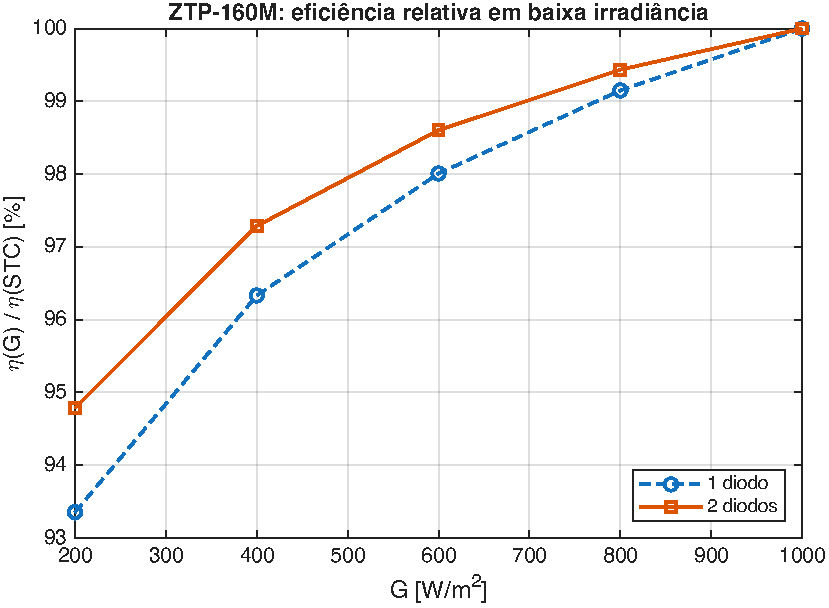
\includegraphics[width=0.49\linewidth]{figs/e1_eficiencia_relativa.pdf}\hfill
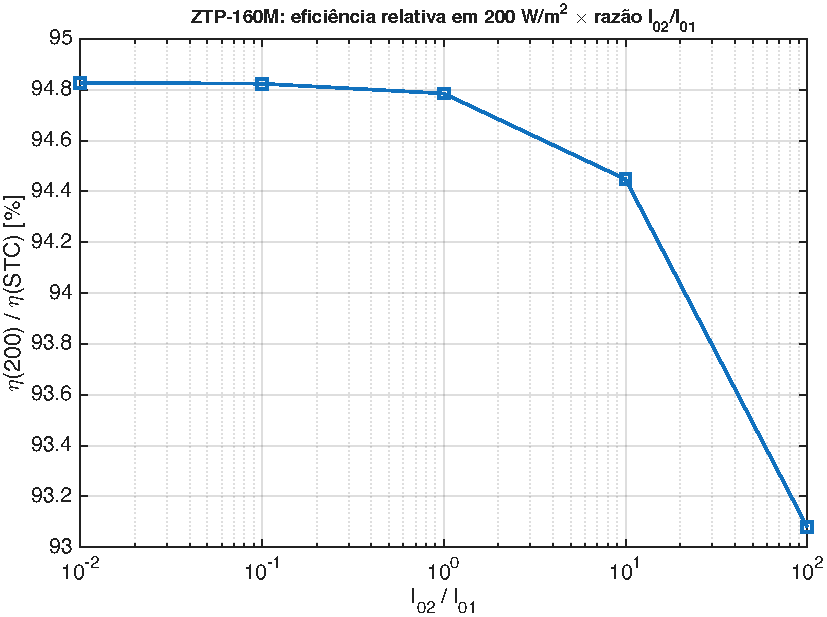
\includegraphics[width=0.49\linewidth]{figs/e1_identificabilidade.pdf}
\caption{(a) Eficiência relativa $\eta(G)/\eta(\mathrm{STC}) = [P_{max}(G)/G]/[P_{max}(1000)/1000]$
do ZTP-160M a 25\,°C, nos modelos de 1 e 2 diodos, ambos com $R_p(G)$; sem curvas medidas, a
figura mostra a diferença entre os modelos e não qual acerta. (b) Eficiência relativa em
200\,W/m² para cada razão $I_{02}/I_{01}$ fixada no ajuste do modelo de 2 diodos (escala
logarítmica): todas fecham as cinco condições do datasheet, mas preveem baixa irradiância de
forma diferente.}
\label{fig:e1}
\end{figure}

\begin{table}[!htbp]
\centering\small
\begin{tabular}{ccccc}
\toprule
$I_{02}/I_{01}$ & Resíduo do ajuste & $E_{g,\mathrm{ef}}$ [eV] & $\eta(200)/\eta(\mathrm{STC})$ &
$\gamma_P$ [\%/K] \\
\midrule
0,01 & $2{,}2\times10^{-11}$ & 1,307 & 0,9483 & $-0{,}362$ \\
0,1  & $2{,}7\times10^{-11}$ & 1,307 & 0,9482 & $-0{,}362$ \\
1    & $4{,}5\times10^{-11}$ & 1,304 & 0,9479 & $-0{,}363$ \\
10   & $4{,}7\times10^{-8}$  & 1,274 & 0,9445 & $-0{,}366$ \\
100  & $2{,}8\times10^{-8}$  & 1,164 & 0,9308 & $-0{,}374$ \\
\bottomrule
\end{tabular}
\caption{Identificabilidade do segundo diodo (\texttt{e1\_identificabilidade.csv}). O
resíduo das cinco condições é praticamente nulo em todas as linhas; a razão 1 é a adotada.}
\label{tab:ident}
\end{table}

\subsection{Modelo térmico}
\label{sec:val_termico}

O NMOT (temperatura nominal de operação do módulo) é a temperatura que o módulo atinge com
800\,W/m², ar a 20\,°C, vento de 1\,m/s e operação no MPP; para o ZTP-160M, 45\,°C. Impondo
$dT/dt = 0$ em \eqref{eq:termico} nessas condições, com $P_{el}$ estimada pelo datasheet,
obtém-se $k_h = 0{,}79$, e a constante de tempo resultante é $\tau \approx 7{,}0$\,min,
dentro da faixa típica de 5 a 7\,min. A primeira versão do modelo usava a correlação de
McAdams ($5{,}7 + 3{,}8\,v_w$), que já inclui a radiação, e mandava as duas faces irradiarem
para o céu; com ela, a calibração exigia $k_h = 0{,}33$, um fator de correção de 3 vezes que
denunciava a radiação contada em dobro. Corrigidas as duas coisas, $k_h$ subiu para 0,79.

\subsection{\texorpdfstring{Modelo chaveado $\times$ modelo médio (E3)}{Modelo chaveado x modelo médio (E3)}}
\label{sec:e3}

A Figura~\ref{fig:e3} compara os dois modelos após um degrau de $+0{,}02$ na razão cíclica.
Em STC (CCM), a média móvel de um período do chaveado segue o modelo médio; no teste de
regressão (painel genérico de 36 células) o desvio máximo ficou em $\sim$0,1\,\% na tensão e
$\sim$0,7\,\% na corrente, e o \emph{ripple} de $i_L$ confere com $\vpv d/(L f_s)$. Em
50\,W/m² a corrente média ($\sim$1\,A) é menor que meio \emph{ripple} ($\sim$3\,A): o indutor
zera a cada período (DCM) e os modelos se separam. Esse é o resultado esperado, e mostra o
limite de validade do modelo médio: em DCM a energia puxada por ciclo é fixada por
$(v\,d\,T_s)^2/(2L)$, o equilíbrio do médio não é equilíbrio do chaveado, e o médio chega a
dar $i_L < 0$. Nas simulações longas a fração de períodos em DCM é registrada: 32\,\% no
perfil EN~50530, que passa muito tempo em irradiâncias baixas, e 13\,\% no dia real.

\begin{figure}[!htbp]
\centering
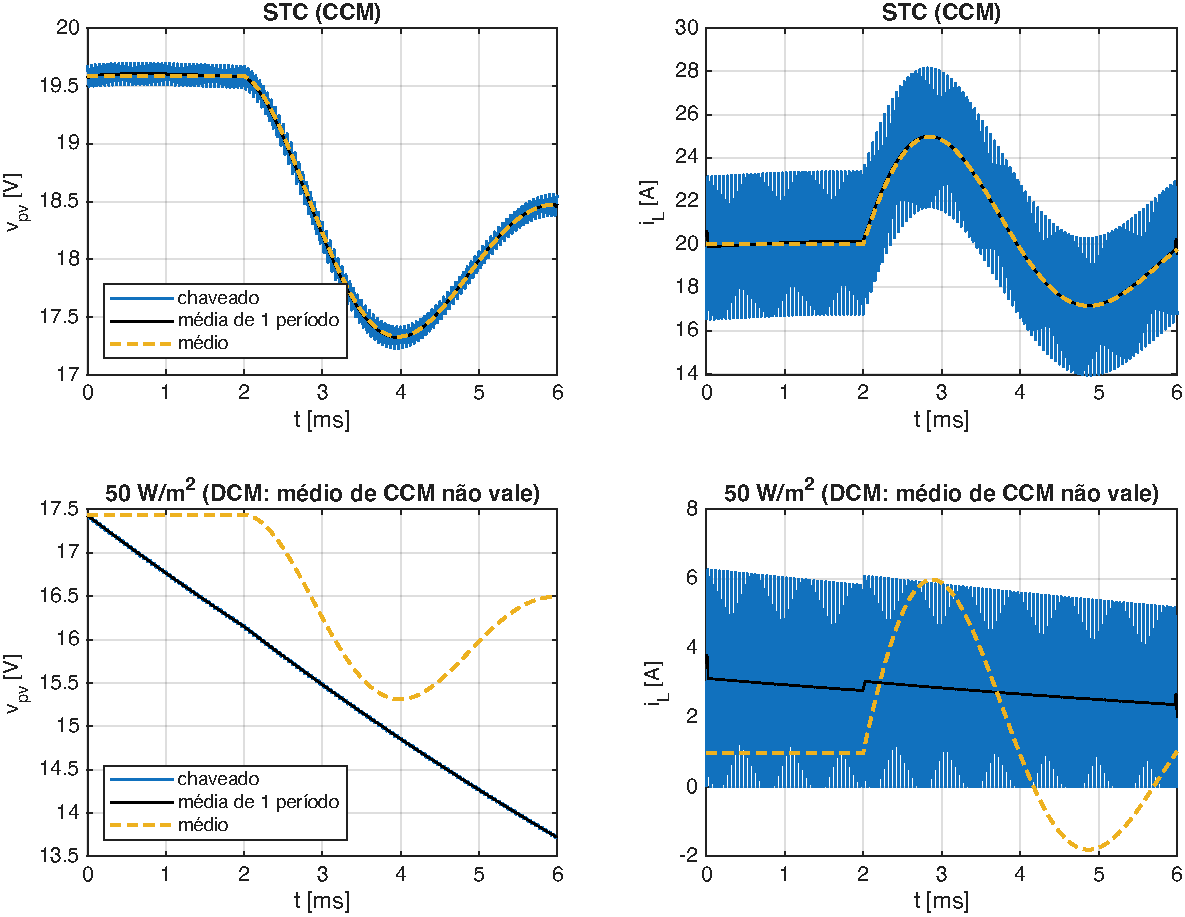
\includegraphics[width=0.82\linewidth]{figs/e3_chaveado_medio.pdf}
\caption{Modelo chaveado (azul, com \emph{ripple}), média móvel de um período do chaveado
(preto) e modelo médio (tracejado laranja) após um degrau de $+0{,}02$ em $d$ em $t = 2$\,ms,
partindo do equilíbrio no MPP. Em cima, STC (1000\,W/m², CCM): o médio acompanha a média do
chaveado em $\vpv$ e $i_L$. Embaixo, 50\,W/m² (DCM): o chaveado mantém $i_L \ge 0$ e
$\vpv$ cai continuamente desde antes do degrau; o médio de CCM não representa esse regime e
chega a $i_L < 0$, fisicamente impossível.}
\label{fig:e3}
\end{figure}

\subsection{Linearização e margens do PI (E4)}

A Figura~\ref{fig:e4bode} mostra a planta e o ganho de malha em todos os casos em CCM. A
Tabela~\ref{tab:margens} resume as margens. A MF é folgada em todos os casos (mínimo de
82,9°), porque o cruzamento fica bem abaixo da ressonância. A MG é o limite do projeto:
o pior caso, 6,2\,dB, ocorre em 200\,W/m², no MPP, com $L$ e $C$ ambos $+20\,\%$ (só com
$L{+}20\,\%$ seriam 6,3\,dB). A margem está a 0,2\,dB do requisito de 6\,dB, e foi
justamente esse requisito que fixou a banda: um PI projetado só com $L$ e $C$ nominais tinha
MG de 4,6\,dB com $L{+}20\,\%$. Um ganho escalonado pelo ponto de operação daria mais folga,
mas ficou fora do escopo.

\begin{figure}[!htbp]
\centering
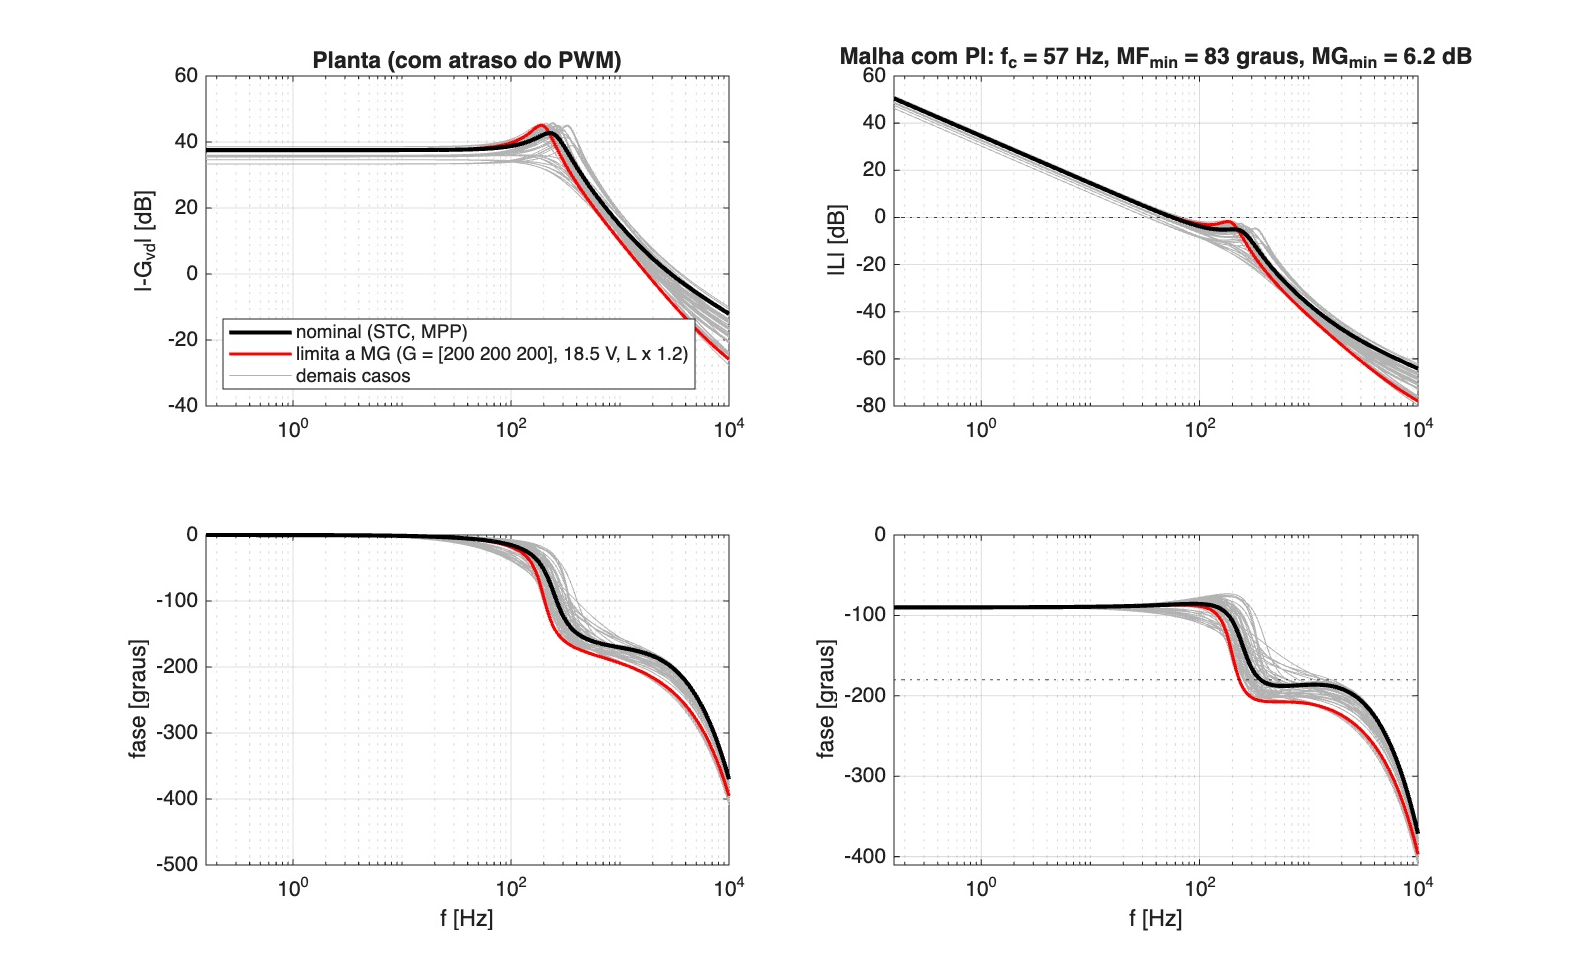
\includegraphics[width=0.92\linewidth]{figs/e4_bode.pdf}
\caption{Diagramas de Bode nos 56 casos de robustez em CCM (12 pontos de operação $\times$
cantos de tolerância de $L$ e $C$). À esquerda, a planta $-G_{vd}$ com o atraso do PWM; à
direita, o ganho de malha com o PI ($f_c = 57$\,Hz). Preto: caso nominal (STC, MPP,
$L$ e $C$ nominais). Vermelho: caso que limita a MG (200\,W/m², 18,5\,V, $L\times1{,}2$;
neste caso também $C\times1{,}2$). Cinza: demais casos. O pico perto de 240\,Hz é a
ressonância LC; a linha pontilhada à direita marca $-180°$.}
\label{fig:e4bode}
\end{figure}

\begin{table}[!htbp]
\centering\small
\begin{tabular}{lcccc}
\toprule
Caso & MF [°] & MG [dB] & $t_s$ [ms] & Observação \\
\midrule
Nominal: 1000\,W/m², MPP (19,6\,V), $L$, $C$ nominais & 93,5 & 15,3 & 12,9 & -- \\
1000\,W/m², 21,5\,V, $L$ e $C$ $+20\,\%$ & \textbf{82,9} & 46,5 & 15,1 & pior MF \\
200\,W/m², MPP (18,5\,V), $L$ e $C$ $+20\,\%$ & 92,7 & \textbf{6,2} & 19,9 & pior MG \\
Sombra $[1\ 1\ 0{,}4]$, pico de 12,7\,V, $L$ e $C$ $-20\,\%$ & 93,7 & 23,1 & \textbf{20,2} &
pior $t_s$ \\
60\,°C, MPP (16,8\,V), $L$, $C$ nominais & 93,7 & 17,5 & 15,2 & -- \\
\bottomrule
\end{tabular}
\caption{Resumo das margens do PI (\texttt{e4\_margens.csv}, 60 casos, 56 em CCM). O pior
$t_s$ ocorre no pico sombreado de baixa tensão, onde o ganho da planta é cerca de 0,6 do
nominal e o cruzamento cai na mesma proporção; ele define $T_a = 1{,}5\times20{,}2 = 31$\,ms.}
\label{tab:margens}
\end{table}

A Figura~\ref{fig:e4degrau} valida a linearização: o degrau de $\Vref$ aplicado ao modelo
linear e ao modelo médio não linear (painel resolvido por Newton, PI com saturação) dá curvas
sobrepostas, tanto no caso nominal quanto no mais lento.

\begin{figure}[!htbp]
\centering
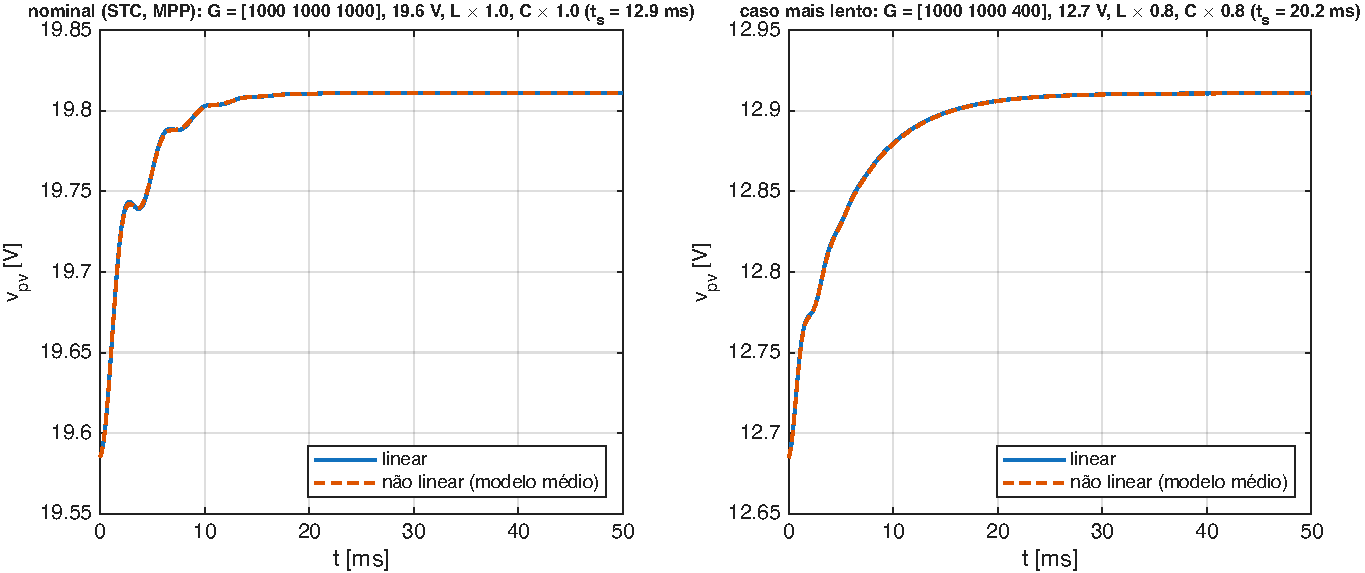
\includegraphics[width=0.92\linewidth]{figs/e4_degrau.pdf}
\caption{Resposta a um degrau de $\Vref$ na malha fechada: modelo linear usado no projeto
(azul) e modelo médio não linear (laranja tracejado). À esquerda, o caso nominal (STC, MPP,
$G = [1000\ 1000\ 1000]$\,W/m², 19,6\,V, $L$ e $C$ nominais; $t_s = 12{,}9$\,ms). À direita,
o caso mais lento (sombra $G = [1000\ 1000\ 400]$\,W/m², pico global de 12,7\,V,
$L\times0{,}8$ e $C\times0{,}8$; $t_s = 20{,}2$\,ms). As ondulações no início da resposta
nominal vêm da ressonância LC pouco amortecida.}
\label{fig:e4degrau}
\end{figure}

\subsection{\texorpdfstring{Quase-estático $\times$ dinâmico}{Quase-estático x dinâmico}}
\label{sec:val_qe}

A hipótese quase-estática foi validada contra a EDO reduzida em cenários de 4 a 20\,s com
um degrau de sombra. Com P\&O e InC a energia do quase-estático difere da dinâmica em
$+0{,}13\,\%$ e $+0{,}14\,\%$. Com o PSO buscando continuamente, a diferença é de $-1{,}1\,\%$,
e numa janela típica de 20\,s (busca de 1 a 2\,s, depois parado no $g_{best}$) cai para
$-0{,}3\,\%$. O sinal negativo tem causa física: depois de um degrau grande de $\Vref$, o
transitório do PI passa por tensões \emph{entre} as partículas, perto do pico, com mais
potência que nas pontas, e o quase-estático só conta a potência em $\Vref$. O erro é,
portanto, \textbf{conservador contra o PSO} e só pesa enquanto ele busca.

A Figura~\ref{fig:e6din} mostra um trecho de duas rampas do perfil EN~50530 no modelo
dinâmico. Rodado também no quase-estático, o mesmo trecho dá $\etaM = 0{,}9988$ (P\&O),
0,9949 (InC) e 0,9762 (PSO), contra 0,999, 0,995 e 0,978 no dinâmico (legenda da figura).
P\&O e InC concordam na terceira casa; o PSO, que reinicia 22 vezes no trecho, fica
0,2 ponto abaixo no quase-estático, no sentido conservador esperado.

\begin{figure}[!htbp]
\centering
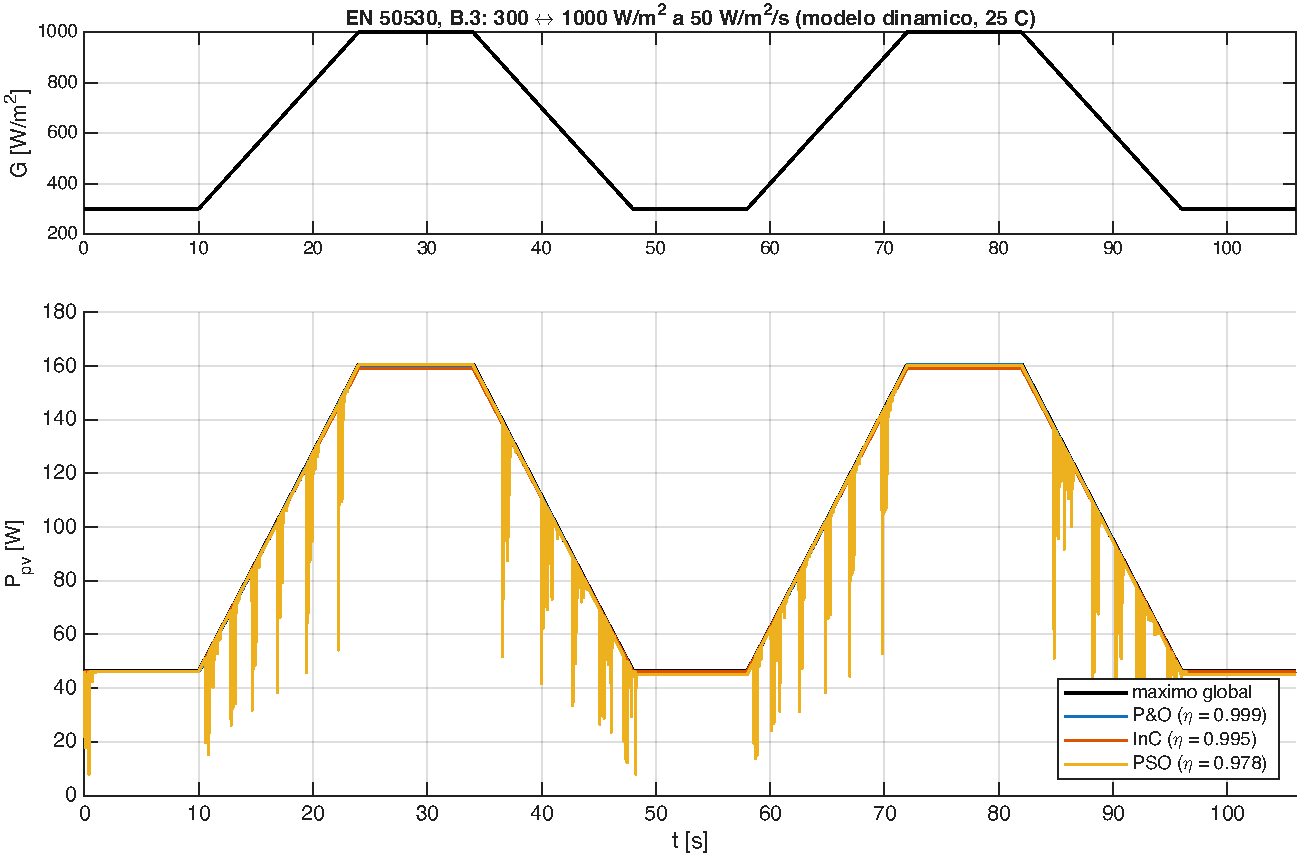
\includegraphics[width=0.9\linewidth]{figs/e6_dinamico.pdf}
\caption{Trecho da sequência B.3 da EN~50530 no modelo dinâmico completo (EDO reduzida),
a 25\,°C, com $\delta = 1\,\%\,V_{oc}$: irradiância uniforme entre 300 e 1000\,W/m² a
50\,W/m²/s (rampas de 14\,s, patamares de 10\,s, dois trapézios; a espera inicial foi
encurtada para 10\,s). Embaixo, a potência do máximo global (preto) e a extraída por cada
algoritmo, com a eficiência $\etaM$ do trecho na legenda. Os ``dentes'' do PSO nas rampas são
reinícios da busca: a cada variação de mais de 10\,\% na potência ele testa as partículas de
novo, passando por tensões de pouca potência.}
\label{fig:e6din}
\end{figure}

% =====================================================================
\section{Resultados}
\label{sec:resultados}

\subsection{Curvas sob sombreamento (E2)}
\label{sec:e2}

A Figura~\ref{fig:e2} e a Tabela~\ref{tab:picos} mostram o efeito do sombreamento no
ZTP-160M a 25\,°C. Sem sombra há um único máximo, de 160,5\,W em 19,6\,V. Com um submódulo a
40\,\%, aparecem dois picos, e o global (103,8\,W) fica em 12,7\,V, \emph{abaixo} da tensão
da bateria; o local de alta tensão, de 70,2\,W em 20,7\,V, é o primeiro que um algoritmo
partindo de perto de $V_{oc}$ encontra. No degradê 100/60/30\,\% aparecem três picos e o
global fica no do meio.

\begin{figure}[!htbp]
\centering
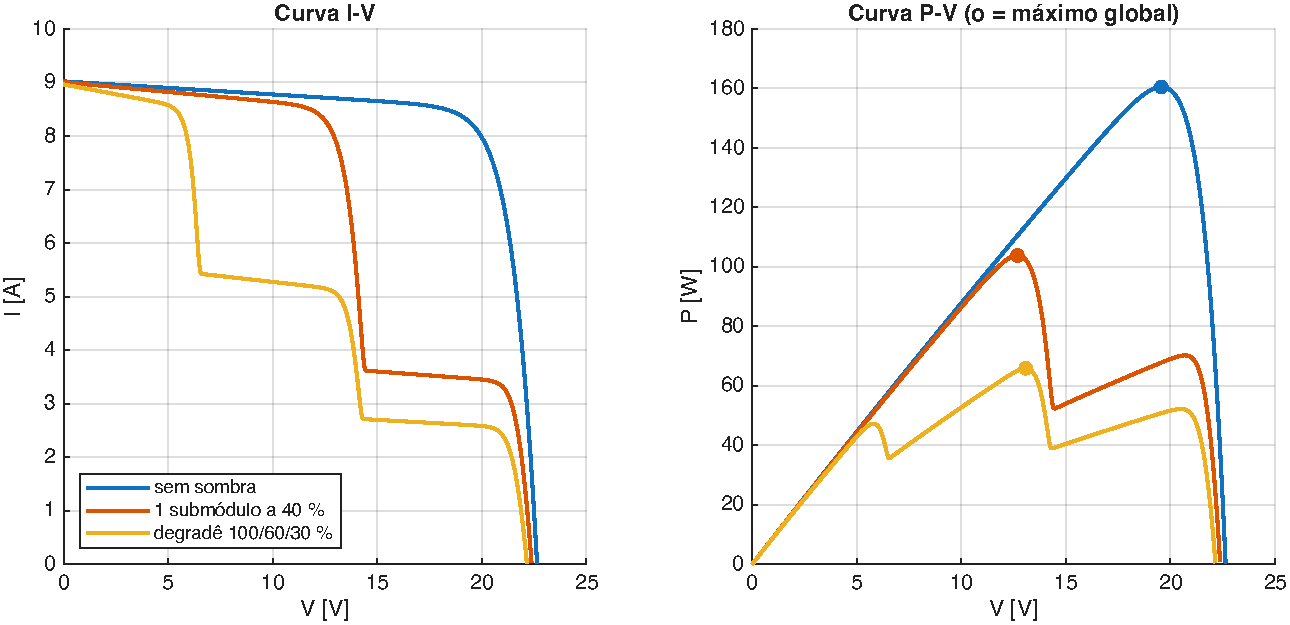
\includegraphics[width=0.95\linewidth]{figs/e2_curvas_sombra.pdf}
\caption{Curvas I-V (esquerda) e P-V (direita) do ZTP-160M a 25\,°C para três padrões de
irradiância por submódulo ($\times1000$\,W/m²): sem sombra (azul), um submódulo a 40\,\%
(laranja) e degradê 100/60/30\,\% (amarelo). As cores da curva P-V são as mesmas da legenda
da curva I-V. Cada degrau da I-V marca a corrente em que um submódulo sombreado entra em
\emph{bypass}; o círculo cheio na P-V marca o máximo global de cada curva.}
\label{fig:e2}
\end{figure}

\begin{table}[!htbp]
\centering\small
\begin{tabular}{lcccc}
\toprule
Padrão ($G_j/1000$) & $V$ [V] & $I$ [A] & $P$ [W] & Global? \\
\midrule
$[1\ 1\ 1]$ & 19,57 & 8,20 & 160,5 & sim \\
\midrule
\multirow{2}{*}{$[1\ 1\ 0{,}4]$} & 12,68 & 8,19 & 103,8 & sim \\
 & 20,69 & 3,39 & 70,2 & não \\
\midrule
\multirow{3}{*}{$[1\ 0{,}6\ 0{,}3]$} & 5,80 & 8,15 & 47,3 & não \\
 & 13,08 & 5,04 & 65,9 & sim \\
 & 20,49 & 2,55 & 52,2 & não \\
\bottomrule
\end{tabular}
\caption{Máximos locais das curvas da Figura~\ref{fig:e2} (\texttt{e2\_picos.csv}).}
\label{tab:picos}
\end{table}

\subsection{Rastreamento sob sombra estática (E5)}

Cada algoritmo rodou 200 períodos $T_a$ sobre o mapa estático do módulo (a tensão é a
referência pedida no passo anterior), em seis padrões de sombra; o PSO, que é aleatório,
rodou com 10 sementes. A Tabela~\ref{tab:e5} mostra a eficiência nos últimos 21 passos.
Nos três padrões em que o pico global não é o de alta tensão, P\&O e InC ficam presos no
pico local: 67\,\%, 79\,\% e 42\,\% do máximo global. Nos outros três, em que o global é o de
alta tensão, eles acertam, e o InC chega mais perto do MPP que o P\&O porque pode parar. O PSO
acha o pico global com as 10 sementes em todos os padrões ($\ge 99{,}99\,\%$), ao custo de 24
a 61 períodos de busca (0,7 a 1,9\,s), contra 1 a 7 dos locais.

\begin{table}[!htbp]
\centering\small
\begin{tabular}{lccccc}
\toprule
Padrão ($G_j/1000$) & Pico global & P\&O & InC & PSO (mín.\ em 10 sementes) &
Passos do PSO \\
\midrule
$[1\ 1\ 1]$         & único       & 0,9989 & 0,9997 & 0,999993 & 24--48 \\
$[1\ 0{,}5\ 0{,}5]$ & alta tensão & 0,9987 & 0,9998 & 0,999995 & 24--48 \\
$[1\ 0{,}3\ 0{,}3]$ & alta tensão & 0,9989 & 0,99997 & 0,999992 & 24--48 \\
$[1\ 1\ 0{,}4]$     & baixa tensão & \textbf{0,6743} & \textbf{0,6759} & 0,999933 & 33--61 \\
$[1\ 0{,}6\ 0{,}3]$ & intermediária & \textbf{0,7902} & \textbf{0,7920} & 0,999944 & 33--61 \\
$[0{,}8\ 0{,}8\ 0{,}2]$ & baixa tensão & \textbf{0,4226} & \textbf{0,4223} & 0,999915 & 33--54 \\
\bottomrule
\end{tabular}
\caption{Eficiência de rastreamento sob sombra estática a 25\,°C
(\texttt{e5\_mppt\_estatico.csv}). O máximo global de referência vem de uma grade de 3000
pontos, por isso algumas sementes do PSO dão $\eta$ ligeiramente acima de 1 (até
$1{,}000001$). Passos do PSO: períodos $T_a$ até a potência ficar a menos de 1\,\% do valor
final (faixa entre as sementes).}
\label{tab:e5}
\end{table}

\subsection{Perfil dinâmico EN 50530 (E6)}

O perfil inteiro ($\approx$7\,h, 352,95\,Wh disponíveis) rodou no quase-estático, a 25\,°C,
com perdas. Para P\&O e InC, o passo $\delta$ foi varrido em 0,5, 1 e 2\,\% de $V_{oc}$
(Tabela~\ref{tab:e6}). O P\&O é melhor com o menor passo ($\etaM = 0{,}9992$): as rampas da
norma são lentas o bastante para o P\&O as seguir mesmo com passos curtos, e a oscilação em
torno do MPP cai com $\delta^2$. O InC tem o comportamento oposto: melhora com o passo e
chega a 0,9958 em $\delta = 2\,\%$, \emph{na borda da faixa varrida}; o ótimo pode estar além
dela, e a comparação com o P\&O fica em aberto nesse ponto. A explicação provável é que o
InC para no MPP: o custo de oscilação que penaliza o passo grande no P\&O quase não existe
nele, e um passo maior só ajuda a seguir as rampas.

O PSO é o pior no perfil (0,9862). Sem sombra a curva tem um só pico e a busca global não
traz ganho; em compensação, a regra de reinício por variação de 10\,\% na potência dispara
2182 vezes nas rampas, e cada busca passa por tensões de pouca potência. Além disso, o
quase-estático é cerca de 1\,\% conservador contra o PSO quando ele busca o tempo todo
(Seção~\ref{sec:val_qe}), o que explica parte da diferença. No trecho dinâmico da
Figura~\ref{fig:e6din} os dentes de cada reinício são visíveis.

\begin{table}[!htbp]
\centering\small
\begin{tabular}{lcccccc}
\toprule
Algoritmo & $\delta$ [\% $V_{oc}$] & $\etaM$ & $E_{pv}$ [Wh] & $E_{bat}$ [Wh] & Reinícios &
DCM [\%] \\
\midrule
P\&O & 0,5 & \textbf{0,9992} & 352,69 & 323,85 & -- & 31,6 \\
P\&O & 1   & 0,9990 & 352,59 & 323,77 & -- & 31,6 \\
P\&O & 2   & 0,9962 & 351,61 & 322,92 & -- & 31,6 \\
InC  & 0,5 & 0,9879 & 348,69 & 319,93 & -- & 29,4 \\
InC  & 1   & 0,9916 & 349,99 & 321,17 & -- & 30,4 \\
InC  & 2   & \textbf{0,9958} & 351,48 & 322,64 & -- & 32,0 \\
PSO  & --  & 0,9862 & 348,08 & 319,67 & 2182 & 31,9 \\
\bottomrule
\end{tabular}
\caption{Perfil dinâmico da EN~50530 (\texttt{e6\_en50530.csv}), irradiância uniforme,
25\,°C, quase-estático com oráculo a cada 1\,s. $E_{max} = 352{,}95$\,Wh. $E_{bat}$ é a
energia entregue à bateria (eficiência média do conversor de $\approx$92\,\%). DCM: fração dos
períodos em condução descontínua.}
\label{tab:e6}
\end{table}

\subsection{Dia real em Florianópolis (E7)}

A Figura~\ref{fig:e7} mostra a potência ao longo do dia com o modelo completo (térmico e
perdas) e a Tabela~\ref{tab:e7} a energia. Os três algoritmos coincidem nas manhãs e tardes
sem sombra. As diferenças aparecem nos eventos. Na sombra de poste (14:00--15:00), P\&O e InC
ficam no pico de alta tensão, com cerca de metade da potência disponível, enquanto o PSO
reinicia, encontra o pico global e o segue. O resultado é $\etaM = 0{,}987$ para o PSO,
contra 0,957 do P\&O e 0,938 do InC. Na bateria, o PSO entrega 941,7\,Wh: 28,3\,Wh (3,1\,\%)
a mais que o P\&O e 45,2\,Wh (5,0\,\%) a mais que o InC. Em energia não captada, isso é
13,8\,Wh para o PSO, 45,7\,Wh para o P\&O e 66,2\,Wh para o InC, de cerca de 1064\,Wh
disponíveis. Os eventos de sombra reduzem a energia disponível de cerca de 1138\,Wh (o
mesmo dia sem eventos, Seção~\ref{sec:e8}) para 1064\,Wh.

\begin{figure}[!htbp]
\centering
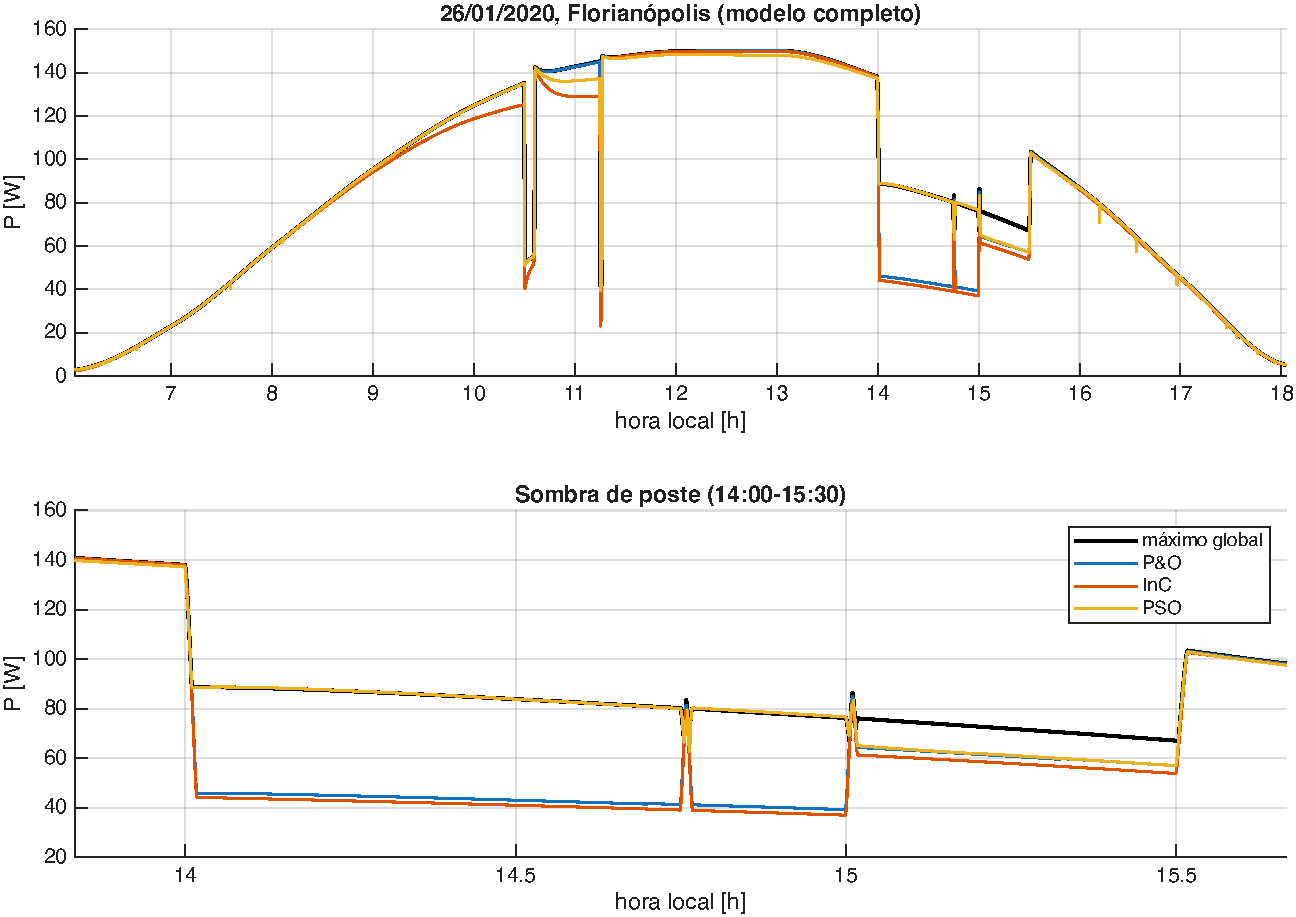
\includegraphics[width=0.92\linewidth]{figs/e7_dia.pdf}
\caption{Dia 26/01/2020 em Florianópolis (PVGIS) com os eventos sintéticos da
Tabela~\ref{tab:eventos}, modelo completo (térmico e perdas, quase-estático). Em cima, o dia
inteiro; embaixo, o detalhe da sombra de poste (14:00--15:30). Preto: máximo global
disponível (oráculo); azul, laranja e amarelo: potência extraída por P\&O, InC e PSO (média
móvel de 20 amostras). Entre 14:00 e 15:00 P\&O e InC ficam no pico local de alta tensão; entre
15:00 e 15:30, com sombra mais fraca e módulo quente, os três ficam abaixo do máximo global
(Seção~\ref{sec:d17}).}
\label{fig:e7}
\end{figure}

\paragraph{Ablação.} O mesmo dia foi simulado sem modelo térmico (células a 25\,°C, como no
trabalho anterior) e sem perdas no conversor (Tabela~\ref{tab:e7}). O módulo chega a
55,6--55,7\,°C; ignorar esse aquecimento aumenta a energia disponível em 9,0\,\% e a energia
na bateria em 8,4 a 9,0\,\%. Ignorar as perdas aumenta a energia na bateria em 11,3 a
11,6\,\%; a eficiência média do conversor no dia é de 89,6 a 89,9\,\%. Os dois efeitos são
maiores que a diferença entre os algoritmos e não mudam o seu ordenamento: \emph{um modelo
isotérmico ou sem perdas erra a energia mais do que a diferença entre o melhor e o pior
algoritmo}.

\begin{table}[!htbp]
\centering\small
\begin{tabular}{llccccc}
\toprule
Variante & Algoritmo & $E_{pv}$ [Wh] & $E_{bat}$ [Wh] & $\etaM$ & $\eta_{conv}$ &
$\Delta E_{bat}$ vs.\ completo \\
\midrule
\multirow{3}{*}{Completo}
 & P\&O & 1018,5 & 913,4 & 0,957 & 0,897 & -- \\
 & InC  & 997,6  & 896,5 & 0,938 & 0,899 & -- \\
 & PSO  & 1050,8 & \textbf{941,7} & \textbf{0,987} & 0,896 & -- \\
\midrule
\multirow{3}{*}{Sem térmico (25\,°C)}
 & P\&O & 1108,8 & 993,7  & 0,956 & 0,896 & $+8{,}8\,\%$ \\
 & InC  & 1091,2 & 976,8  & 0,941 & 0,895 & $+9{,}0\,\%$ \\
 & PSO  & 1143,7 & 1020,8 & 0,986 & 0,893 & $+8{,}4\,\%$ \\
\midrule
\multirow{3}{*}{Sem perdas}
 & P\&O & 1018,5 & 1018,5 & 0,957 & 1 & $+11{,}5\,\%$ \\
 & InC  & 997,6  & 997,6  & 0,938 & 1 & $+11{,}3\,\%$ \\
 & PSO  & 1050,8 & 1050,8 & 0,987 & 1 & $+11{,}6\,\%$ \\
\bottomrule
\end{tabular}
\caption{Energia no dia 26/01/2020 com eventos sintéticos e ablação (\texttt{e7\_dia.csv}).
$E_{max}$ (máximo global integrado) é 1064\,Wh com o térmico e 1160\,Wh a 25\,°C. Reinícios do
PSO: 104 no completo e 107 sem térmico. Fração de períodos em DCM: 13\,\%.}
\label{tab:e7}
\end{table}

\subsection{O que só o modelo completo revela}
\label{sec:d17}

Três limitações dos algoritmos só aparecem com o modelo térmico e o dia real. Elas não foram
corrigidas, de propósito: são resultados da modelagem, e um modelo mais simples as
esconderia.
\begin{enumerate}[label=(\roman*)]
\item \textbf{O PSO não acompanha a deriva térmica.} Depois de convergir, o PSO fixa a
referência no $g_{best}$. Após a nuvem das 10:30, o módulo esquenta de 43 para 53\,°C, o
$V_{mp}$ desce com a temperatura e o PSO fica 3 a 4\,\% abaixo do máximo, sem reiniciar,
porque a potência muda menos de 10\,\%. Com temperatura fixa, como no trabalho anterior, o
$V_{mp}$ não se moveria e o efeito não existiria.
\item \textbf{O InC congela.} Parado no MPP, o InC só sai do lugar quando a corrente varia
mais de 0,2\,\% de $I_{sc}$ por amostra ($\approx$18\,mA em 31\,ms). As variações lentas do
dia (sol e temperatura) nunca atingem esse limiar, e o InC fica parado enquanto o MPP se
desloca. É por isso que, no dia real, o InC é o pior dos três, embora sob sombra estática
seja o mais preciso dos locais.
\item \textbf{Sombra fraca em módulo quente engana o PSO.} Às 15:00, com sombra
$[1\ 1\ 0{,}5]\times656$\,W/m² e módulo a 44\,°C, o pico global está em 11,6\,V e o local em
18,9\,V. As posições iniciais do PSO, calculadas com o $V_{mp}$ de STC, ficam mal colocadas
para essa curva, e o enxame converge no pico local. O efeito aparece na
Figura~\ref{fig:e7} entre 15:00 e 15:30.
\end{enumerate}
As correções são conhecidas e ficam como trabalho futuro: reverificação periódica no PSO
(uma pequena perturbação local depois de convergir, ou um reinício por tempo), posições
iniciais corrigidas pela temperatura medida e, no InC, um limiar de corrente proporcional à
irradiância.

\subsection{O trabalho anterior como linha de base (E8)}
\label{sec:e8}

Para medir o efeito conjunto das simplificações do trabalho anterior, o mesmo dia, sem os
eventos de sombra, foi simulado com dois modelos, ambos com P\&O e o mesmo PI: o
``anterior'' (1 diodo, conversor ideal, células a 25\,°C) e o completo (2 diodos, perdas,
térmico). A Tabela~\ref{tab:e8} mostra que o anterior superestima a energia na bateria em
21,9\,\%.

\begin{table}[!htbp]
\centering\small
\begin{tabular}{lccccc}
\toprule
Modelo & $E_{pv}$ [Wh] & $E_{bat}$ [Wh] & $\etaM$ & $T_{max}$ [°C] & $\Delta E_{bat}$ \\
\midrule
Anterior (1 diodo, ideal, 25\,°C) & 1238,4 & 1238,4 & 0,9991 & 25,0 & $+21{,}9\,\%$ \\
Completo (2 diodos, perdas, térmico) & 1137,2 & 1015,8 & 0,9991 & 55,6 & -- \\
\bottomrule
\end{tabular}
\caption{Linha de base do trabalho anterior no dia 26/01/2020 sem sombras, com P\&O
(\texttt{e8\_baseline.csv}). $\Delta E_{bat}$: diferença relativa ao modelo completo.}
\label{tab:e8}
\end{table}

A diferença se decompõe de forma multiplicativa. As perdas do conversor respondem por
$1137{,}2/1015{,}8 = 1{,}120$ ($+12\,\%$). O restante, $1238{,}4/1137{,}2 = 1{,}089$ ($+9\,\%$),
reúne a temperatura e a troca de 2 para 1 diodo. Como só a temperatura já aumenta a energia
disponível em 9,0\,\% no E7, a contribuição do modelo de 1 diodo é praticamente nula. Isso
é coerente com o E1: os dois modelos são ajustados aos mesmos pontos do datasheet e diferem
pouco perto do STC, onde está quase toda a energia de um dia de verão. O erro do trabalho
anterior não estava no número de diodos, mas no que ficou fora do modelo.

% =====================================================================
\section{Conclusão}
\label{sec:conclusao}

\paragraph{Resposta à pergunta central.} Sob sombreamento parcial estático, o P\&O pode
perder de 21 a 58\,\% da potência disponível, conforme o padrão de sombra (eficiências de
79\,\% a 42\,\%), porque para no pico local; o PSO recupera praticamente tudo
($\ge 99{,}99\,\%$). Num dia real de verão em Florianópolis com uma hora de sombra de poste e
duas nuvens, considerando o aquecimento do módulo (até 55,6\,°C) e as perdas do conversor, o
P\&O deixa de captar 45,7\,Wh (4,3\,\% da energia disponível) e o PSO, 13,8\,Wh (1,3\,\%); na
bateria, o PSO entrega 3,1\,\% a mais que o P\&O e 5,0\,\% a mais que o InC. A busca global tem
um custo: sem sombra, no perfil EN~50530, o PSO perde 1,3 ponto de eficiência para o P\&O,
porque reinicia a cada rampa. O PSO compensa quando há sombras que deslocam o pico global, e
não compensa quando o céu só varia de forma uniforme.

\paragraph{Sobre a modelagem.} Os resultados que mais pesam na energia não vêm dos
algoritmos: ignorar o aquecimento superestima a energia em cerca de 9\,\% e ignorar as perdas
do conversor, em cerca de 11\,\%; juntas, as simplificações do trabalho anterior dão
$+21{,}9\,\%$. Do lado dos métodos, o trabalho mostrou que (i) o datasheet não identifica o
segundo diodo e o gap precisa ser efetivo, (ii) $R_p(G)$ corrige uma perda de 26\,\% em baixa
irradiância sem significado físico, (iii) a DAE com matriz de massa falha em 9 de 36 casos e a
EDO reduzida resolve o problema, e (iv) a hierarquia chaveado $\to$ médio $\to$
quase-estático, validada em cada degrau, permite simular as 13\,h de sol em 10 a 25\,min de
CPU. A modelagem
completa também expôs limitações dos algoritmos que um modelo isotérmico esconderia
(Seção~\ref{sec:d17}).

\paragraph{Limitações.}
\begin{itemize}
\item A ruptura reversa das células \citep{bishop} não é modelada; como o \emph{bypass}
conduz muito antes da ruptura, o efeito sobre a curva é pequeno, mas o aquecimento local
(\emph{hot spot}) fica fora do modelo.
\item O número de diodos de \emph{bypass} é uma hipótese: o datasheet informa a associação
``3$\times$11'' das 33 células, mas não quantos diodos há; adotaram-se 3 submódulos de 11
células, a configuração usual.
\item A temperatura do módulo é uniforme: um submódulo sombreado, na realidade, fica mais
frio que os outros.
\item A bateria é uma fonte ideal de 12\,V; a tensão não varia com o estado de carga.
\item As sombras e nuvens do E7 são sintéticas, e os dados do PVGIS são horários; os
resultados de energia valem para esse cenário, não para um dia típico.
\item O modelo quase-estático é cerca de 1\,\% conservador contra o PSO enquanto ele busca;
no perfil EN~50530, em que ele busca com frequência, a eficiência do PSO pode estar
subestimada nessa ordem.
\item A MG do PI é de 6,2\,dB no pior caso, a 0,2\,dB do requisito, e o modelo médio de CCM
não descreve os 13 a 32\,\% do tempo em DCM, onde as perdas de condução são subestimadas.
\item Os valores das perdas do conversor são típicos de catálogo, não de um protótipo; a
ablação mostra o tamanho do seu efeito, não o seu valor exato.
\end{itemize}

\paragraph{Trabalho futuro.} Reverificação periódica e posições iniciais corrigidas pela
temperatura no PSO; limiar de corrente proporcional à irradiância no InC; varredura do passo
do InC além de 2\,\%\,$V_{oc}$; ganho escalonado no PI; modelo de DCM; temperatura por
submódulo; e validação experimental com curvas I-V medidas do ZTP-160M.

\section*{Disponibilidade do código}
O código MATLAB, os testes automatizados, os dados de entrada e as tabelas de resultados
(\texttt{resultados/*.csv}) que geram todas as figuras e tabelas deste relatório estão no
repositório do trabalho.

\bibliographystyle{elsarticle-harv}
\bibliography{referencias}

\end{document}
